\documentclass[aspectratio=169,11pt]{beamer}

% ── Tema e colori ──────────────────────────────────────────────────────
\usetheme{Madrid}
\usecolortheme{default}
\definecolor{uniblue}{RGB}{0,60,113}
\setbeamercolor{structure}{fg=uniblue}
\setbeamercolor{title}{fg=white,bg=uniblue}
\setbeamercolor{frametitle}{fg=white,bg=uniblue}
\setbeamercolor{block title}{fg=white,bg=uniblue}
\setbeamercolor{block body}{bg=uniblue!5}
\setbeamercolor{item}{fg=uniblue}
\setbeamertemplate{navigation symbols}{}
\setbeamertemplate{footline}{%
  \leavevmode\hbox{%
    \begin{beamercolorbox}[wd=.33\paperwidth,ht=2.5ex,dp=1ex,center]{author in head/foot}%
      \usebeamerfont{author in head/foot}\insertshortauthor
    \end{beamercolorbox}%
    \begin{beamercolorbox}[wd=.34\paperwidth,ht=2.5ex,dp=1ex,center]{title in head/foot}%
      \usebeamerfont{title in head/foot}\insertshorttitle
    \end{beamercolorbox}%
    \begin{beamercolorbox}[wd=.33\paperwidth,ht=2.5ex,dp=1ex,right]{date in head/foot}%
      \hspace*{2ex}
    \end{beamercolorbox}}%
  \vskip0pt%
}

% ── Pacchetti ──────────────────────────────────────────────────────────
\usepackage[utf8]{inputenc}
\usepackage[T1]{fontenc}
\usepackage[italian]{babel}
\usepackage{amsmath,amssymb}
\usepackage{booktabs}
\usepackage{graphicx}
\usepackage{tikz}
\usepackage{multirow}
\usepackage{colortbl}
\usepackage{xcolor}
\usepackage{adjustbox}

% ── Metadata ───────────────────────────────────────────────────────────
\title[Arricchimento Semantico e Unlearning]{%
  {\normalsize Elaborato di Laurea in Informatica}\\[0.5em]
  {\Large Arricchimento Semantico e Unlearning}}
\author[A.\ Gambalonga]{Alberto Gambalonga\texorpdfstring{\\[0.2em]}{, }
  {\small Matricola 0124002583}}
\institute[UniParthenope]{%
  Universit\`a degli Studi di Napoli ``Parthenope''\\[0.3em]
  Corso di Laurea in Informatica\\[0.5em]
  {\small Relatore: Ch.mo Prof.\ Antonio Maratea}}
\date{Anno Accademico 2024--2025}

% ======================================================================
\begin{document}

% ── SLIDE 1: Titolo ───────────────────────────────────────────────────
\begin{frame}[plain]
  \titlepage
\end{frame}

% ── SLIDE 2: Contesto e Motivazione ──────────────────────────────────
\begin{frame}{Contesto e Motivazione}
  \begin{columns}[T]
    \begin{column}{0.55\textwidth}
      \begin{itemize}
        \item I \textbf{Large Language Models} apprendono da enormi corpora web
        \item Memorizzano inevitabilmente informazioni \textbf{indesiderate}:
          \begin{itemize}
            \item Dati personali (GDPR, diritto all'oblio)
            \item Contenuti protetti da copyright
            \item Bias, disinformazione, conoscenze pericolose
          \end{itemize}
        \item L'informazione è \textbf{distribuita} su milioni di parametri\\[0.3em]
        \item Riaddestrare da zero è \textbf{computazionalmente proibitivo}
      \end{itemize}
    \end{column}
    \begin{column}{0.42\textwidth}
      \begin{block}{Machine Unlearning LLM}
        Rimuovere selettivamente la conoscenza appresa \textbf{senza} riaddestrare il modello, preservando le capacità generali.
      \end{block}
      \vspace{0.5em}
      \begin{alertblock}{Problema aperto}
        Molte tecniche producono un forgetting \textbf{apparente}: l'informazione resta recuperabile con interrogazioni riformulate.
      \end{alertblock}
    \end{column}
  \end{columns}
\end{frame}

% ── SLIDE 3: Formulazione del Problema ───────────────────────────────
\begin{frame}{Formulazione del Problema}
  \begin{columns}[T]
    \begin{column}{0.55\textwidth}
      Definiamo due insiemi:
      \begin{itemize}
        \item $\textcolor{red}{D_f}$: \textbf{Forget set} — dati da dimenticare
        \item $\textcolor{red}{D_r}$: \textbf{Retain set} — conoscenza da preservare
      \end{itemize}
      \vspace{0.4em}
      Dato un modello $\theta$ \textcolor{red}{addestrato su $D_f \cup D_r$},\\
      obiettivo: trovare $\theta_{\mathrm{unl}}$ tale che:
      \[
        \min_{\theta} \left\{
          -\mathcal{L}_f(\theta) + \lambda\,\mathcal{L}_r(\theta)
        \right\}
      \]
      \begin{itemize}
        \item Massimizzare la loss sul forget set
        \item Minimizzare la loss sul retain set
        \item $\lambda$: trade-off forgetting vs.\ retention
      \end{itemize}
    \end{column}
    \begin{column}{0.42\textwidth}
      \begin{block}{Vincoli}
        \begin{enumerate}
          \item $\theta_{\mathrm{unl}} \approx \theta_{\mathrm{ret}}$\\
                {\small (indistinguibile dal retraining)}
          \item Invarianza delle capacità generali
        \end{enumerate}
      \end{block}
      \vspace{0.5em}
      \begin{exampleblock}{Sfida centrale}
        Eliminare troppo $\rightarrow$ degrado globale\\
        Eliminare troppo poco $\rightarrow$ forgetting apparente
      \end{exampleblock}
    \end{column}
  \end{columns}
\end{frame}

% ── SLIDE 4: Metodi di Unlearning ────────────────────────────────────
\begin{frame}{Stato Dell'Arte - Metodi di Unlearning}
  \begin{columns}[T]
    \begin{column}{0.31\textwidth}
      \begin{block}{\small Ascesa del Gradiente}
        \scriptsize
        Invertono il processo di apprendimento: massimizzano la loss su $D_f$.
        \vspace{0.5em}
        \begin{itemize}\setlength{\itemsep}{4pt}
          \item \textbf{GradDiff}:\\ascesa su $D_f$ + regolarizzazione su $D_r$
        \end{itemize}
        \vspace{0.5em}
        {\tiny \textcolor{red}{Rischio}: collasso catastrofico se non regolarizzati.}
      \end{block}
    \end{column}
    \hfill
    \begin{column}{0.34\textwidth}
      \begin{block}{\small Ottimizzazione di Preferenze}
        \scriptsize
        Guidano il modello a \textbf{preferire} risposte alternative a quelle da dimenticare.
        \vspace{0.5em}
        \begin{itemize}\setlength{\itemsep}{4pt}
          \item \textbf{DPO}: preferisce risposta evasiva vs.\ corretta
          \item \textbf{NPO}: solo preferenza negativa, senza alternative
          \item \textbf{SimNPO}: come NPO ma senza modello di riferimento
        \end{itemize}
        \vspace{0.5em}
        {\tiny \textcolor{teal}{Pi\`u stabili} e output pi\`u coerenti.}
      \end{block}
    \end{column}
    \hfill
    \begin{column}{0.31\textwidth}
      \begin{block}{\small Rappresentazioni / Distillazione}
        \scriptsize
        Agiscono sulle \textbf{rappresentazioni interne}, senza invertire il gradiente.
        \vspace{0.5em}
        \begin{itemize}\setlength{\itemsep}{4pt}
          \item \textbf{RMU}: sovrascrive le attivazioni di $D_f$ con rumore casuale $\Rightarrow$ la conoscenza diventa illeggibile
          \item \textbf{UNDIAL}: il modello si ri-addestra sulla propria distribuzione con i logit delle risposte da dimenticare attenuati
        \end{itemize}
        \vspace{0.5em}
        {\tiny \textcolor{teal}{Nessuna massimizzazione} $\Rightarrow$ convergenza stabile.}
      \end{block}
    \end{column}
  \end{columns}
\end{frame}

% ── SLIDE 5: Domanda di Ricerca ──────────────────────────────────────
\begin{frame}{Domanda di Ricerca}
  \begin{center}
    \Large
    \textit{L'introduzione di \textbf{parafrasi} durante l'unlearning\\[0.3em]
    può rendere il forgetting più \textbf{robusto}\\[0.3em]
    e \textbf{semanticamente} profondo?}
  \end{center}
  \vspace{1em}
  \begin{columns}[T]
    \begin{column}{0.48\textwidth}
      \begin{block}{Stato dell'arte}
        Le parafrasi sono usate solo come \textbf{strumento di valutazione} post-unlearning per smascherare forgetting superficiale.
      \end{block}
    \end{column}
    \begin{column}{0.48\textwidth}
      \begin{block}{Metodo proposto}
        Integrare le parafrasi \textbf{direttamente nel processo} di unlearning, costringendo il modello a dimenticare a livello \textbf{semantico}.
      \end{block}
    \end{column}
  \end{columns}
\end{frame}

% ── SLIDE 5: S-UNL — Pipeline ────────────────────────────────────────
\begin{frame}{S-UNL: Semantic-Unlearning LLM}
  \begin{columns}[T]
    \begin{column}{0.55\textwidth}
      \centering
      
\includegraphics[width=\textwidth]{img/s_unl_arch.jpg}
    \end{column}
    \begin{column}{0.43\textwidth}
      \small
      \begin{enumerate}
        \item \textbf{Data Loader}\\[0.1em]
              Genera offline fino a 20 parafrasi per domanda $\rightarrow$ $D_f^{\text{para}}$
        \vspace{0.3em}
        \item \textbf{Unlearning Engine}\\[0.1em]
              Applica il metodo scelto sul modello di partenza usando il dataset arricchito
        \vspace{0.3em}
        \item \textbf{Evaluator}\\[0.1em]
              Valutazione su 3 assi: memorizzazione, privacy, utilit\`a
      \end{enumerate}
    \end{column}
  \end{columns}
\end{frame}

% ── SLIDE 6: Setup Sperimentale ──────────────────────────────────────
\begin{frame}{Setup Sperimentale}
  \vspace{-0.5em}
  \begin{columns}[T]
    \begin{column}{0.48\textwidth}
      \begin{block}{Benchmark \& Modello}
        \scriptsize
        \begin{itemize}\setlength{\itemsep}{0pt}
          \item \textbf{TOFU} (\textit{Task of Fictitious Unlearning}):
                dataset sintetico di 200 autori fittizi
          \item \texttt{forget10}: 20 autori, 400 coppie Q\&A
          \item \textbf{Llama-3.2-1B-Instruct\_Full}, LR=$10^{-5}$, 20 ep., bs 32
        \end{itemize}
      \end{block}
      \vspace{-0.1em}
      \begin{block}{Configurazioni parafrasi}
        \centering
        \scriptsize
        \begin{tabular}{lrc}
          \toprule
          Config & \#Esempi & Fattore \\
          \midrule
          para0  & 400   & 1$\times$ \\
          para5  & 2\,400 & 6$\times$ \\
          para10 & 4\,400 & 11$\times$ \\
          para15 & 6\,400 & 16$\times$ \\
          para20 & 8\,400 & 21$\times$ \\
          \bottomrule
        \end{tabular}
      \end{block}
    \end{column}
    \begin{column}{0.48\textwidth}
      \begin{block}{Metodi di Unlearning (6)}
        \small
        \textbf{Ottimizzazione di preferenze}
        \begin{itemize}\setlength{\itemsep}{1pt}
          \item DPO (Direct Preference Opt.)
          \item NPO (Negative Preference Opt.)
          \item SimNPO (Simplified NPO)
        \end{itemize}
        \textbf{Approcci alternativi}
        \begin{itemize}\setlength{\itemsep}{1pt}
          \item GradDiff (Gradient Difference)
          \item RMU (Representation Misdirection)
          \item UNDIAL (Self-Distillation)
        \end{itemize}
      \end{block}
    \end{column}
  \end{columns}
\end{frame}

% ── SLIDE 7: Metriche di Valutazione ─────────────────────────────────
\begin{frame}{Metriche di Valutazione}
  \vspace{-0.3em}
  \begin{columns}[T]
    \begin{column}{0.32\textwidth}
      \begin{block}{\small Memorizzazione $\downarrow$}
        \scriptsize
        \begin{itemize}\setlength{\itemsep}{2pt}
          \item \textbf{Exact Mem.\ (EM)}: fraz.\ token riprodotti letteralmente
          \item \textbf{Extr.\ Strength (ES)}: facilit\`a di completamento da prefisso minimo
          \item \textbf{Probability}: confidenza nella risposta corretta (anche parafrasata)
          \item \textbf{Truth Ratio}: discrimina corretta vs.\ perturbata\\
                {\tiny Ideale $\approx 0.5$ = indecisione}
        \end{itemize}
      \end{block}
    \end{column}
    \begin{column}{0.32\textwidth}
      \begin{block}{\small Privacy ($\approx\!0.5$)}
        \scriptsize
        \begin{itemize}\setlength{\itemsep}{2pt}
          \item \textbf{MIA} (Loss, Min-K++): AUC membership inference attack
          \item \textbf{Priv.\ Leakage}: informazione residua deducibile\\
                {\tiny Ideale $\approx 0$}
        \end{itemize}
        \vspace{0.3em}
        \scriptsize AUC $= 0.5$ $\Rightarrow$ forget e holdout \textbf{indistinguibili}
      \end{block}
    \end{column}
    \begin{column}{0.32\textwidth}
      \begin{block}{\small Utilit\`a $\uparrow$}
        \scriptsize
        \begin{itemize}\setlength{\itemsep}{2pt}
          \item \textbf{Model Utility (MU)}: prestazioni su retain set e task generali
          \item \textbf{Forget Fluency (FF)}: coerenza linguistica risposte su forget set
        \end{itemize}
        \vspace{0.3em}
        \scriptsize \textbf{MU$\times$FF}: score combinato
      \end{block}
    \end{column}
  \end{columns}
  \vspace{0.4em}
  \begin{center}
    \small Un modello idealmente \textit{unlearned} deve risultare \textbf{indistinguibile} da uno mai addestrato su $D_f$.
  \end{center}
\end{frame}

% ── SLIDE 8: Risultati — Memorizzazione ──────────────────────────────
\begin{frame}{Risultati: Memorizzazione Letterale}
  \vspace{-0.5em}
  \centering
  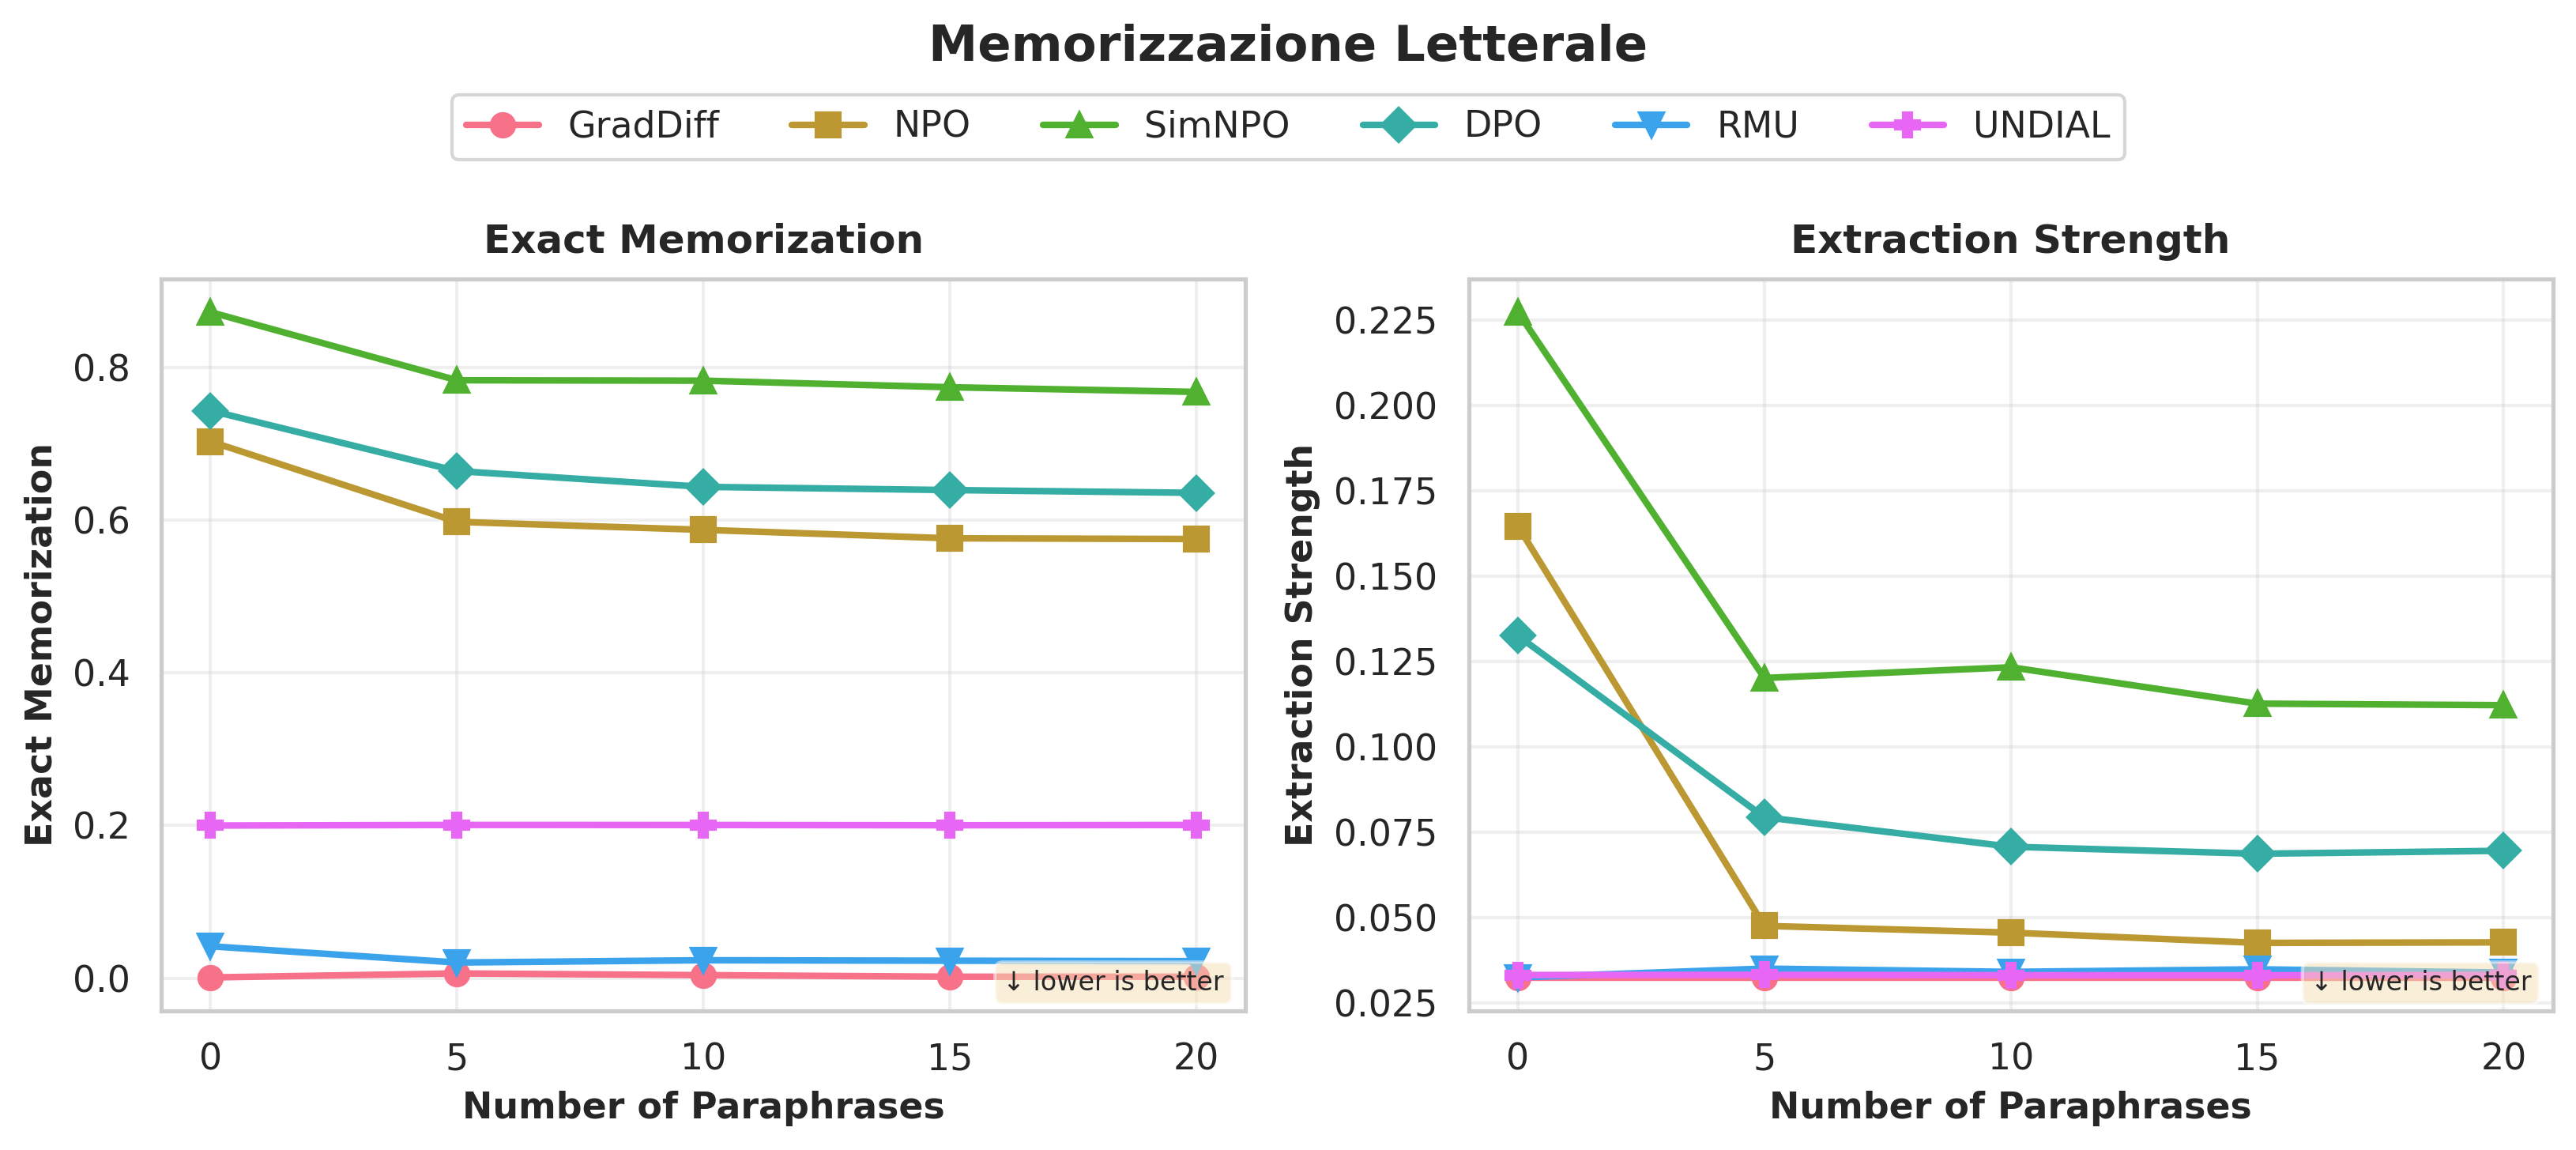
\includegraphics[width=0.82\textwidth]{img/composite/memorizzazione_letterale.png}
  \vspace{-0.2em}
  \begin{columns}[T]
    \begin{column}{0.48\textwidth}
      \begin{itemize}
        \scriptsize
        \item EM: NPO \textcolor{teal}{--18.2\%}, DPO \textcolor{teal}{--14.5\%}, SimNPO \textcolor{teal}{--12\%}
        \item GradDiff/RMU gi\`a $\approx 0$ alla baseline: operano sulle rappresentazioni interne
      \end{itemize}
    \end{column}
    \begin{column}{0.48\textwidth}
      \begin{itemize}
        \scriptsize
        \item ES: NPO \textcolor{teal}{--74\%}, SimNPO \textcolor{teal}{--51\%}, DPO \textcolor{teal}{--48\%}
        \item UNDIAL \textbf{insensibile}: teacher congelato $\Rightarrow$ nessun segnale utile
      \end{itemize}
    \end{column}
  \end{columns}
\end{frame}

% ── SLIDE 7b: Trend Memorizzazione ────────────────────────────────────

% ── SLIDE 8: Risultati — Probabilità e Truth Ratio ───────────────────
\begin{frame}{Risultati: Memorizzazione Semantica}
  \vspace{-0.5em}
  \centering
  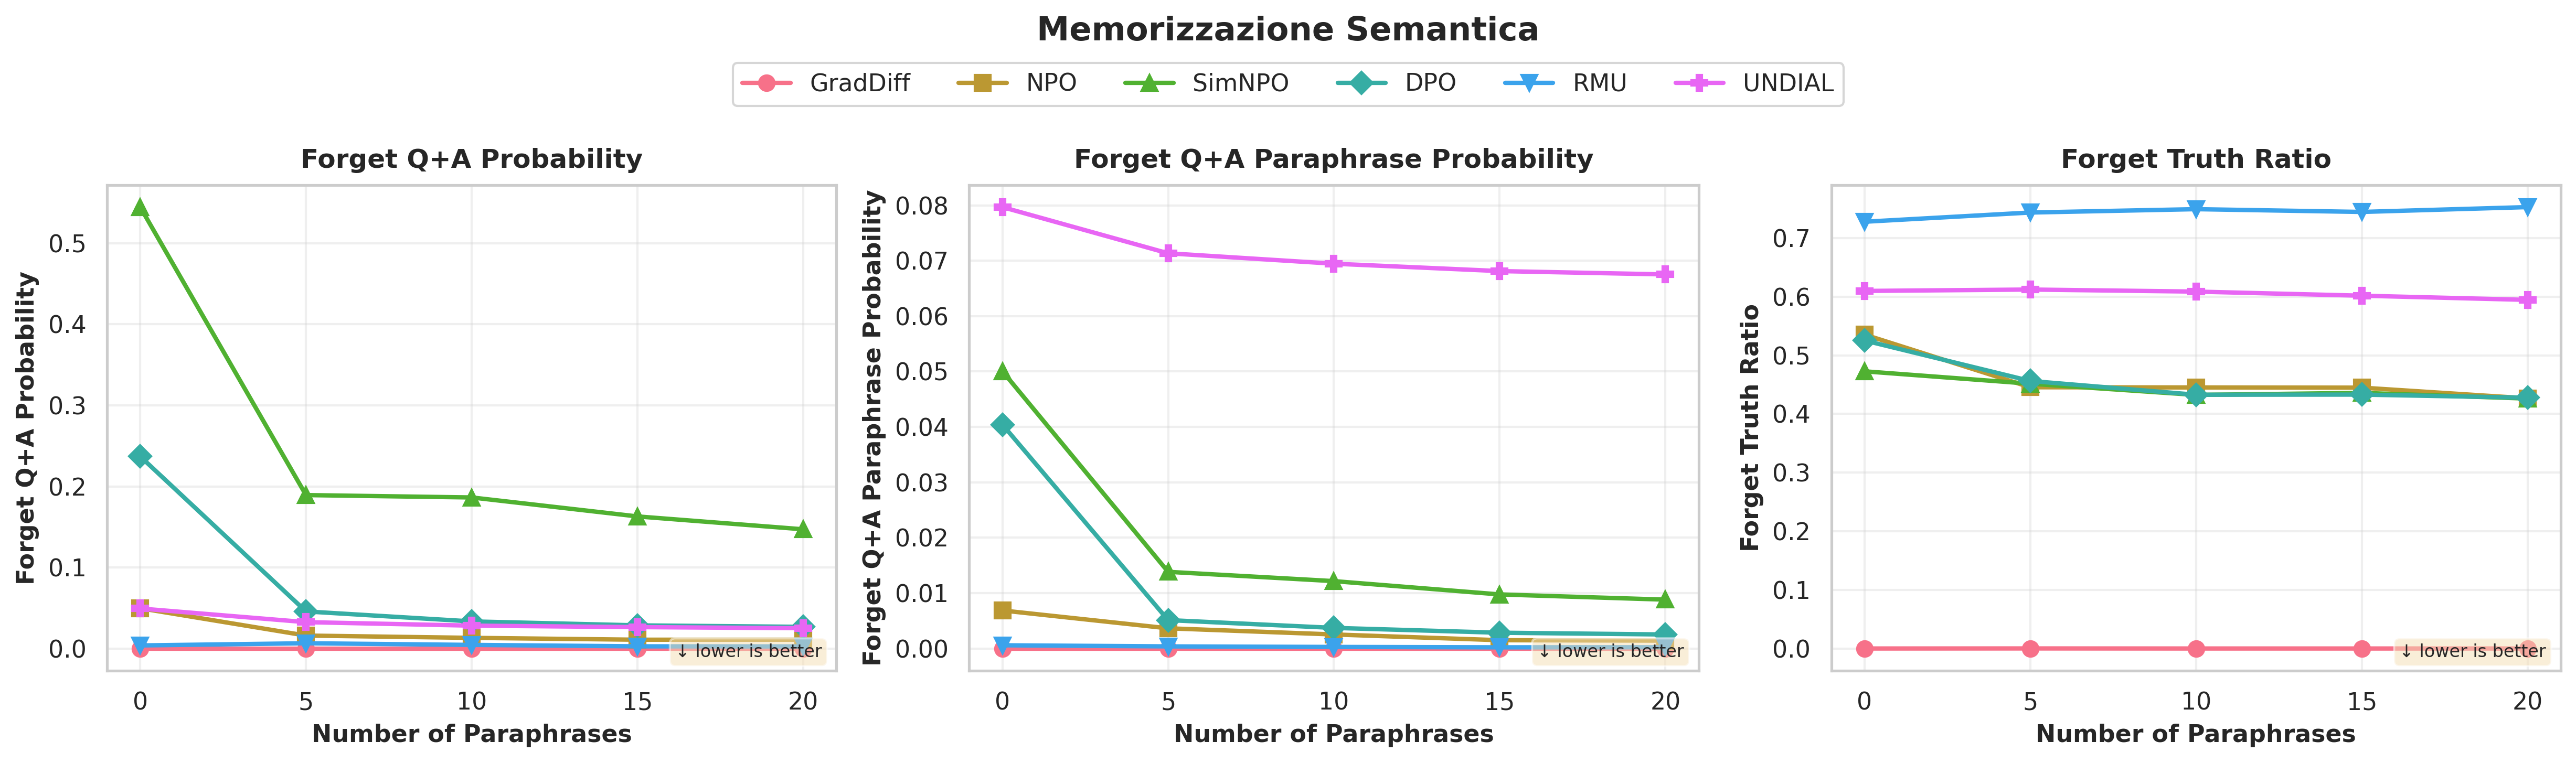
\includegraphics[width=0.82\textwidth]{img/composite/memorizzazione_semantica.png}
  \vspace{-0.2em}
  \begin{alertblock}{Evidenza chiave}
    \scriptsize DPO: Prob originale \textcolor{teal}{--88.7\%}, Prob parafrasata \textcolor{teal}{--93.7\%}. Il Truth Ratio converge a $\approx 0.5$ per DPO, NPO, SimNPO $\Rightarrow$ perdita della capacit\`a discriminativa.
  \end{alertblock}
\end{frame}

% ── SLIDE 9: Risultati — Privacy (MIA) ──────────────────────────────
\begin{frame}{Risultati: Privacy — Membership Inference Attacks}
  \vspace{-0.5em}
  \centering
  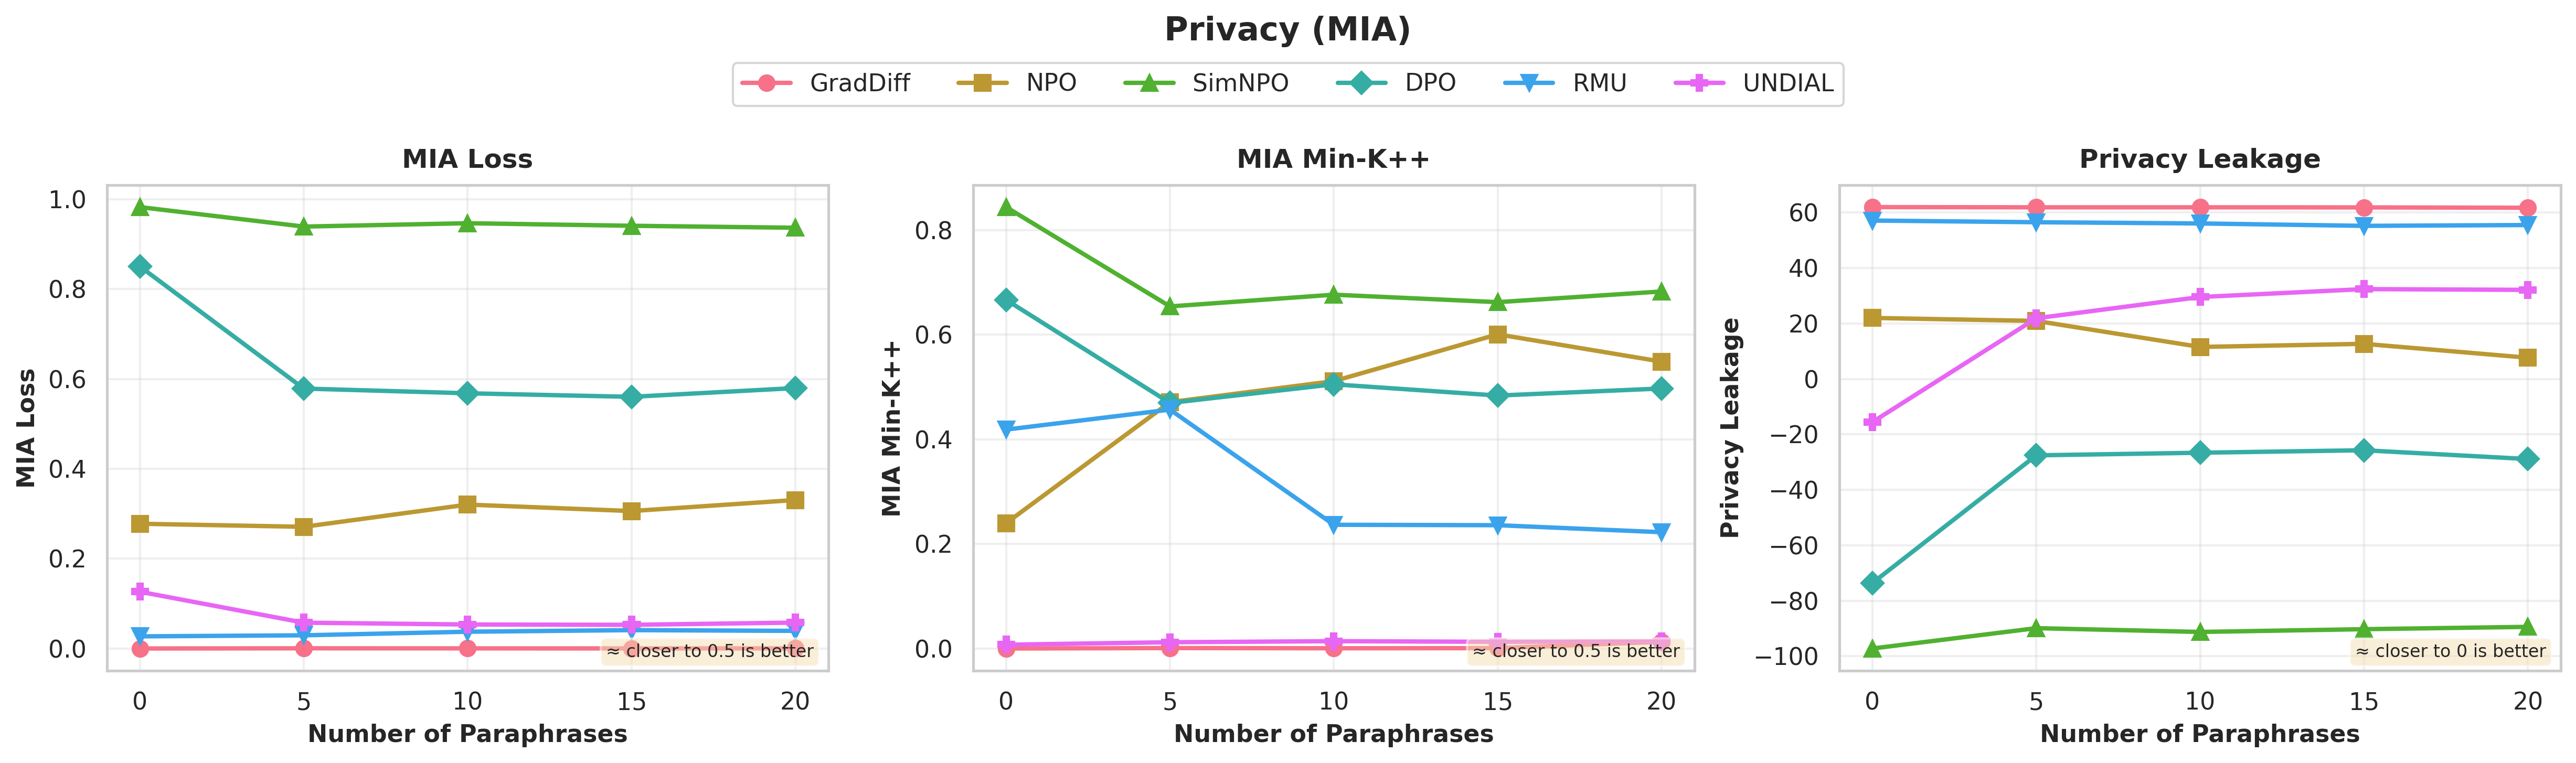
\includegraphics[width=0.82\textwidth]{img/composite/privacy_mia.png}
  \vspace{-0.2em}
  \begin{block}{Interpretazione}
    \scriptsize AUC $\approx 0.5$ = \textcolor{teal}{\textbf{indistinguibile}}. \textbf{DPO} con para20: tutte le varianti in $[0.48,\, 0.58]$. GradDiff/RMU: segnali atipici, non correggibili.
  \end{block}
\end{frame}

% ── SLIDE 10: Risultati — Utilità e Fluency ──────────────────────────
\begin{frame}{Risultati: Utilit\`a e Forget Fluency}
  \vspace{-0.5em}
  \centering
  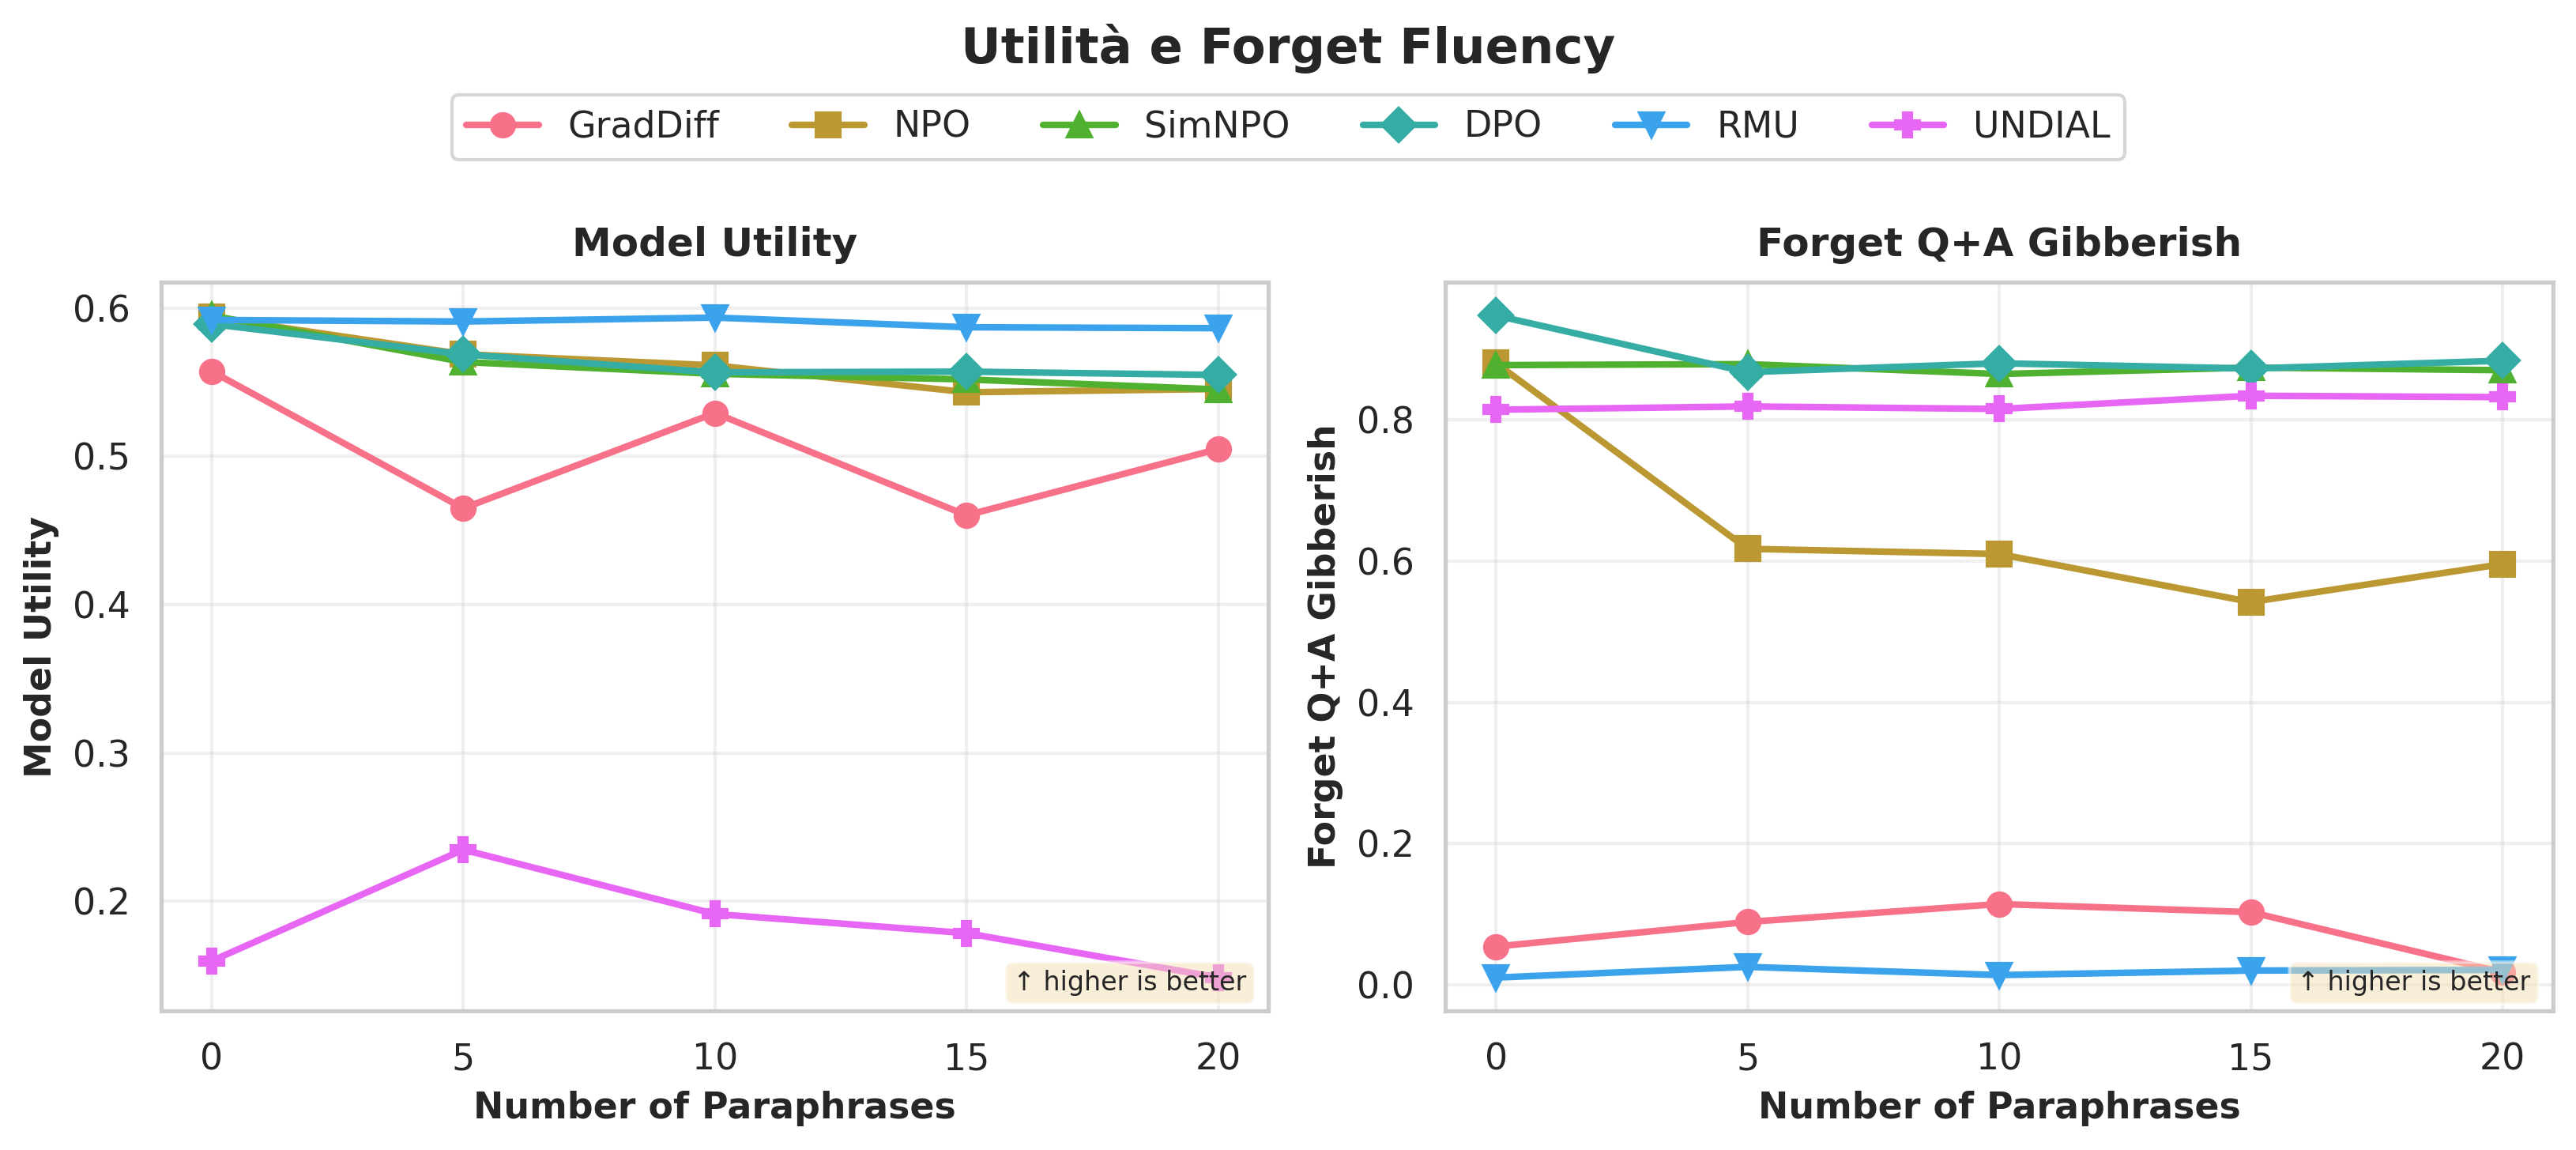
\includegraphics[width=0.82\textwidth]{img/composite/utilita_forget_fluency.png}
  \vspace{-0.2em}
  \begin{columns}[T]
    \begin{column}{0.32\textwidth}
      \begin{alertblock}{Risultato chiave}
        \scriptsize RMU/GradDiff: ottima MU ma \textbf{gibberish} ($>$97\%).
      \end{alertblock}
    \end{column}
    \begin{column}{0.32\textwidth}
      \begin{exampleblock}{Deployment}
        \scriptsize \textbf{DPO}/\textbf{SimNPO}: forgetting + risposte \textbf{fluide}.
      \end{exampleblock}
    \end{column}
    \begin{column}{0.32\textwidth}
      \begin{block}{MU$\times$FF}
        \scriptsize
        DPO: \textbf{0.491} | SimNPO: 0.475\\[0.1em]
        NPO: 0.325 | RMU: 0.012
      \end{block}
    \end{column}
  \end{columns}
\end{frame}

% ── SLIDE 12: Sintesi dei Risultati ──────────────────────────────────
\begin{frame}{Sintesi dei Risultati Principali}
  \begin{columns}[T]
    \begin{column}{0.48\textwidth}
      \begin{block}{1. Le parafrasi funzionano}
        Riducono memorizzazione letterale \textbf{e} semantica.
      \end{block}
      \vspace{0.3em}
      \begin{block}{2. Effetto metodo-dipendente}
        \begin{itemize}
          \small
          \item \textbf{DPO}: miglior bilanciamento complessivo
          \item \textbf{GradDiff/RMU}: già ottimali, ma output degradato
          \item \textbf{UNDIAL}: insensibile (teacher congelato)
        \end{itemize}
      \end{block}
    \end{column}
    \begin{column}{0.48\textwidth}
      \begin{block}{3. Privacy migliorata}
        DPO converge a indistinguibilità statistica (AUC $\approx$ 0.5) su tutte le varianti MIA.
      \end{block}
      \vspace{0.3em}
      \begin{block}{4. Forget Fluency \`e cruciale}
        Un modello che genera \textbf{gibberish} non \`e deployabile. DPO/SimNPO mantengono risposte fluide.
      \end{block}
      \vspace{0.3em}
      \begin{block}{5. 5--10 parafrasi bastano}
        Rendimenti decrescenti: il guadagno si satura rapidamente.
      \end{block}
    \end{column}
  \end{columns}
\end{frame}

% ── SLIDE 14: Conclusioni e Sviluppi Futuri ──────────────────────────
\begin{frame}{Conclusioni e Sviluppi Futuri}
  \begin{columns}[T]
    \begin{column}{0.50\textwidth}
      \begin{block}{Contributo principale}
        L'integrazione di parafrasi nel processo di unlearning non è un semplice aumento quantitativo dei dati, ma un intervento \textbf{qualitativo} che modifica il livello a cui opera la rimozione della conoscenza.
      \end{block}
      \vspace{0.3em}
      \begin{exampleblock}{Implicazioni pratiche}
        \begin{itemize}
          \item 5--10 parafrasi: costo $\sim$10--20h vs.\ $\sim$2h baseline
          \item DPO/SimNPO consigliati per deployment reali
        \end{itemize}
      \end{exampleblock}
    \end{column}
    \begin{column}{0.47\textwidth}
      \begin{alertblock}{Sviluppi futuri}
        \begin{itemize}
          \item Scalabilità a modelli $>$7B parametri
          \item Validazione su dataset realistici (MUSE, WMDP)
          \item Criteri automatici di selezione delle parafrasi
        \end{itemize}
      \end{alertblock}
    \end{column}
  \end{columns}
\end{frame}

% ── SLIDE 15: Chiusura ───────────────────────────────────────────────
\begin{frame}[plain]
  \begin{center}
    \vspace{2cm}
    {\Huge\color{uniblue} Grazie per l'attenzione}\\[1.5em]
    {\Large Domande?}\\[2em]
    {\normalsize
      \textbf{Alberto Gambalonga} — Matricola 0124002583\\[0.3em]
      Universit\`a degli Studi di Napoli ``Parthenope''\\[0.3em]
      Relatore: Ch.mo Prof.\ Antonio Maratea\\[0.5em]
      Codice: \url{https://github.com/agambalonga/S-UNL}
    }
  \end{center}
\end{frame}

% ======================================================================
% APPENDICE — Dettaglio Metriche (slide di backup per domande)
% ======================================================================

% ── BACKUP 1: Memorizzazione Letterale ────────────────────────────────
\begin{frame}{Appendice: Memorizzazione Letterale}
  \scriptsize
  \begin{block}{Exact Memorization (EM) $\downarrow$}
    \textit{Quanto il modello copia parola per parola la risposta originale.}\\[0.3em]
    Frazione di token rigenerati letteralmente rispetto alla ground truth $y$:
    \[
      EM = \frac{1}{|y|} \sum_{k=1}^{|y|}
      \mathbf{1}\!\left(
        \arg\max_{v \in \mathcal{V}} p(v \mid x, y_{<k}; \theta) = y_k
      \right)
    \]
  \end{block}
  \vspace{-0.3em}
  \begin{block}{Extraction Strength (ES) $\downarrow$}
    \textit{Quanto basta dare un piccolo suggerimento per far emergere tutta la risposta memorizzata.}\\[0.3em]
    Prefisso minimo $k$ per rigenerare il suffisso $y_{\geq k}$:
    \[
      ES = 1 - \frac{1}{|y|} \min_{k} \left\{ k \mid f([x, y_{<k}]; \theta) = y_{\geq k} \right\}
    \]
    \vspace{-0.1em}
    {\tiny ES alto $\Rightarrow$ bastano poche parole iniziali per ricostruire l'intera risposta.}
  \end{block}
\end{frame}

% ── BACKUP 2: Memorizzazione Semantica ───────────────────────────────
\begin{frame}{Appendice: Memorizzazione Semantica}
  \scriptsize
  \begin{block}{Probability / Paraphrased Prob $\downarrow$}
    \textit{Quanto il modello \`e sicuro della risposta corretta (anche riformulata).}\\[0.3em]
    $P = p(y \mid x;\theta) = \prod_{k=1}^{|y|} p(y_k \mid x, y_{<k}; \theta)$
    \hfill $P_{\text{para}}$: stessa formula su $y_{\text{para}}$\\[0.3em]
    {\tiny Dopo un buon unlearning, il modello non dovrebbe essere pi\`u sicuro della risposta corretta.}
  \end{block}
  \vspace{-0.3em}
  \begin{block}{Truth Ratio $\approx 0.5$}
    \textit{Il modello preferisce ancora la risposta vera a una falsa?}\\[0.3em]
    $\text{TR} = \dfrac{p(y_{\text{para}} \mid x;\theta)}{p(y_{\text{para}} \mid x;\theta) + p(y_{\text{pert}} \mid x;\theta)}$\\[0.5em]
    \begin{tabular}{@{}ll@{}}
      $p(y_{\text{para}}) \gg p(y_{\text{pert}})$ & $\rightarrow$ TR $\approx 1$ — sa ancora distinguere vero da falso\\
      $p(y_{\text{para}}) \approx p(y_{\text{pert}})$ & $\rightarrow$ TR $\approx 0.5$ — \textbf{ideale}: non sa pi\`u quale \`e corretta\\
      $p(y_{\text{pert}}) \gg p(y_{\text{para}})$ & $\rightarrow$ TR $\approx 0$ — preferisce il falso (over-unlearning)
    \end{tabular}
  \end{block}
\end{frame}

% ── BACKUP 3: Metriche di Privacy ────────────────────────────────────
\begin{frame}{Appendice: Metriche di Privacy}
  \vspace{-0.8em}
    \tiny
  \begin{block}{\tiny MIA Loss $\approx 0.5$}
    \textit{Un attaccante pu\`o capire se un dato era nel training guardando quanto bene il modello lo predice?}\\[0.2em]
    $s_{\text{LOSS}}(x, y) = \frac{1}{|y|} \sum_{i=1}^{|y|}
    \mathcal{L}_{\text{CE}}\!\bigl(f(x, y_{<i}; \theta),\, y_i\bigr)$
    \hfill Loss bassa $\Rightarrow$ alta confidenza $\Rightarrow$ possibile memorizzazione. AUC $= 0.5$: indistinguibile.
  \end{block}
  \vspace{-0.8em}
  \begin{block}{\tiny MIA Min-K++ $\approx 0.5$}
    \textit{Variante pi\`u robusta: normalizza per evitare falsi allarmi da token rari.}\\[0.2em]
    $z_i = \dfrac{\log p_\theta(y_i \mid x, y_{<i}) - \mu_i}{\sqrt{\sigma_i^2 + \epsilon}}$
    \quad poi \quad
    $s_{\text{Min-K\!+\!+}} = -\dfrac{1}{K}\!\sum_{i \in \mathcal{K}_K(z)} z_i$
  \end{block}
  \vspace{-0.8em}
  \begin{block}{\tiny Privacy Leakage (PrivLeak)}
    \textit{Deviazione \% della privacy del modello unlearned rispetto al retrained (gold standard).}\\[0.2em]
    $\mathrm{PrivLeak} =
    \frac{(1 - \mathrm{AUC}_{unl}) - (1 - \mathrm{AUC}_{ret})}
         {(1 - \mathrm{AUC}_{ret})} \times 100
    = \frac{\mathrm{AUC}_{ret} - \mathrm{AUC}_{unl}}
           {1 - \mathrm{AUC}_{ret}} \times 100$\\[0.2em]
    $(1\!-\!\mathrm{AUC})$ misura la protezione: AUC$=0.5 \Rightarrow$ max privacy, AUC$=1 \Rightarrow$ zero privacy.\\[0.1em]
    $\approx 0\%$: stessa privacy del retrained (ideale) \quad
    $> 0\%$: pi\`u privato del retrained (possibile over-unlearning) \quad
    $< 0\%$: meno privato, unlearning incompleto
  \end{block}
\end{frame}

% ── BACKUP 4: Metriche di Utilità ────────────────────────────────────
\begin{frame}{Appendice: Metriche di Utilit\`a}
  \scriptsize
  \begin{block}{Model Utility (MU) $\uparrow$}
    \textit{Il modello sa ancora rispondere alle domande che NON deve dimenticare?}\\[0.3em]
    Media armonica di 9 sotto-metriche su retain set, real authors, world facts:
    \vspace{-0.3em}
    \[
      \text{MU} = \text{HM}\!\left(
        P_{\text{ret}}, R_{\text{ret}}, T_{\text{ret}},\;
        P_{\text{ra}}, R_{\text{ra}}, T_{\text{ra}},\;
        P_{\text{wf}}, R_{\text{wf}}, T_{\text{wf}}
      \right)
    \]
    \vspace{-0.1em}
    {\tiny $P$ = Probability, $R$ = ROUGE-L, $T$ = Truth Ratio. MU bassa = il modello ha perso troppe capacit\`a generali.}
  \end{block}
  \vspace{-0.3em}
  \begin{block}{Forget Fluency (FF) $\uparrow$}
    \textit{Le risposte sul forget set sono ancora frasi sensate o sono gibberish?}\\[0.3em]
    $\text{FF} = \frac{1}{|D_f|} \sum_{(x,y) \in D_f}
    \mathbf{1}\!\Big(\text{Clf}\!\big(f(x;\theta)\big) = \text{``coerente''}\Big)$
    \hfill {\tiny Classificatore binario coerente/gibberish.}
  \end{block}
  \vspace{-0.3em}
  \begin{block}{MU$\times$FF — Score Complessivo}
    \textit{Bilancia capacit\`a generali e qualit\`a dell'output in un'unica metrica.}\\[0.3em]
    $\text{Score} = \text{MU} \times \text{FF}$
    \hfill DPO: \textbf{0.491} | SimNPO: 0.475 | NPO: 0.325 | RMU: 0.012
  \end{block}
\end{frame}

% ── BACKUP 5: Metodi — Ascesa del Gradiente ──────────────────────────
\begin{frame}{Appendice: Metodi basati sull'Ascesa del Gradiente}
  \scriptsize
  \begin{block}{Gradient Ascent (GA)}
    \textit{Il metodo pi\`u semplice: invertire il segno del gradiente per massimizzare la loss su $D_f$.}\\[0.3em]
    $\mathcal{L}_{GA}(\theta) = -\,\mathcal{L}_{CE}(\theta;\, D_f)$\\[0.3em]
    {\tiny Nessun vincolo di preservazione $\Rightarrow$ rischio elevato di \textbf{collasso catastrofico}: il modello genera testo incoerente dopo pochi passi.}
  \end{block}
  \vspace{-0.3em}
  \begin{block}{Gradient Difference (GradDiff)}
    \textit{Aggiunge un termine di regolarizzazione sul retain set per arginare il collasso.}\\[0.3em]
    $\mathcal{L}_{GD}(\theta) = -\,\mathcal{L}_{CE}(\theta;\, D_f) \;+\; \lambda \cdot \mathcal{L}_{CE}(\theta;\, D_r)$\\[0.3em]
    {\tiny Due segnali contrapposti: allontanarsi da $D_f$ e restare vicini a $D_r$. Il parametro $\lambda$ controlla il bilanciamento.}
  \end{block}
  \vspace{-0.3em}
  \begin{alertblock}{Limite comune}
    La massimizzazione diretta della loss \`e intrinsecamente instabile: il paesaggio della funzione obiettivo non \`e limitato superiormente e l'ottimizzazione pu\`o divergere.
  \end{alertblock}
\end{frame}

% ── BACKUP 6: Metodi — Ottimizzazione di Preferenze ─────────────────
\begin{frame}{Appendice: Metodi basati sull'Ottimizzazione di Preferenze}
  \scriptsize
  \begin{block}{DPO (Direct Preference Optimization)}
    \textit{Il modello impara a preferire una risposta evasiva rispetto a quella corretta da dimenticare.}\\[0.3em]
    $\mathcal{L}_{DPO}(\theta) = -\,\mathbb{E}\!\left[\log \sigma\!\left(\beta \log \frac{\pi_\theta(y_w \mid x)}{\pi_{\mathrm{ref}}(y_w \mid x)} - \beta \log \frac{\pi_\theta(y_l \mid x)}{\pi_{\mathrm{ref}}(y_l \mid x)}\right)\right]$\\[0.3em]
    {\tiny $y_w$: risposta desiderata (evasiva), $y_l$: risposta da dimenticare. Richiede la preparazione di risposte alternative.}
  \end{block}
  \vspace{-0.3em}
  \begin{block}{NPO (Negative Preference Optimization)}
    \textit{Solo preferenza negativa: basta dire cosa NON deve dire, senza fornire alternative.}\\[0.3em]
    $\mathcal{L}_{NPO}(\theta) = -\frac{2}{\beta}\,\mathbb{E}\!\left[\log \sigma\!\left(-\beta \log \frac{\pi_\theta(y \mid x)}{\pi_{\mathrm{ref}}(y \mid x)}\right)\right]$\\[0.3em]
    {\tiny Il rapporto con $\pi_{\mathrm{ref}}$ frena la divergenza $\Rightarrow$ collasso esponenzialmente pi\`u lento di GA.}
  \end{block}
  \vspace{-0.3em}
  \begin{block}{SimNPO (Simplified NPO)}
    \textit{Elimina il modello di riferimento, evitando il reference model bias.}\\[0.3em]
    $\mathcal{L}_{SimNPO}(\theta) = -\frac{2}{\beta}\,\mathbb{E}\!\left[\log \sigma\!\left(-\frac{\beta}{|y|}\, \log \pi_\theta(y \mid x)\right)\right]$\\[0.3em]
    {\tiny La normalizzazione per $|y|$ bilancia sequenze di lunghezza diversa.}
  \end{block}
\end{frame}

\end{document}
